%% LyX 2.1.4 created this file.  For more info, see http://www.lyx.org/.
%% Do not edit unless you really know what you are doing.
\documentclass[12pt,english]{article}
\usepackage[T1]{fontenc}
\usepackage[utf8x]{inputenc}
\usepackage{geometry}
\geometry{verbose,tmargin=2cm,bmargin=2cm,lmargin=3cm,rmargin=2cm,headheight=2cm,headsep=2cm}
\usepackage{amsmath}
\usepackage{amsthm}
\usepackage{amssymb}
\usepackage{graphicx}
\usepackage{setspace}
\doublespacing

\makeatletter
%%%%%%%%%%%%%%%%%%%%%%%%%%%%%% Textclass specific LaTeX commands.
\numberwithin{equation}{section}
\numberwithin{figure}{section}
\theoremstyle{plain}
\newtheorem{thm}{\protect\theoremname}
  \theoremstyle{definition}
  \newtheorem{defn}[thm]{\protect\definitionname}
  \theoremstyle{plain}
  \newtheorem{prop}[thm]{\protect\propositionname}

%%%%%%%%%%%%%%%%%%%%%%%%%%%%%% User specified LaTeX commands.
\usepackage{babel}
\usepackage{algorithmic}

\makeatother

\usepackage{babel}
  \providecommand{\definitionname}{Definition}
  \providecommand{\propositionname}{Proposition}
\providecommand{\theoremname}{Theorem}

\begin{document}

\title{\textbf{Quantifying the effect of synchrony on the persistence of
infectious diseases in a metapopulation}}


\author{\textbf{Tran Thi Cam Giang, Marc Choisy, Jean-Daniel Zucker, Yann
Chevaleyre}}


\date{\textbf{25/2/2016}}
\maketitle
\begin{abstract}
Global persistence of infectious diseases is a big problem for epidemiologists.
Studies have showed that there are a lot of reasons to answer why
many communicable diseases still exist and have been developed in
more dangerous form. The asynchrony and the recolonization among subpopulations
are two key reasons pointed out. However, why these are the asynchrony
and the recolonozations in a metapopulation is still an open question.
Here we study the combined effects of forcing phase heterogeneity
in the seasonally forced contact rate on global persistence of disease.
We carry out an exploitation of stochastic dynamics in a susceptible-exposed-infectious-recovered
(SEIR) model of the spread of infectious diseases in a metapopulation
of $n$ subpopulations. Starting with continuous-time Markov description
of the model of deterministic equation, the direct method of Gillespie(1977)
\cite{gillespie1977exact} in the class of Monte-Carlo simulation
methods allows us to simulate exactly the spread of disease with the
SEIR model. Our finding of the exploitation of stochastic dynamics
points out that the persistence of the disease in the metapopulation
is characterized as an exponential survival model on data simulated
by the stochastic model. Using a parametric survival model for an
exponential distribution (R package 'survival' \cite{survival-package}),
we estimate the global extinction rate which represents the global
persistence of disease in the meta-population. Besides, we estimate
the locale extinction rate and the recolonization rate in metapopulation
by using the Poisson process. We find how bigger the forcing phase
heterogeneity becomes, and how smaller the local extinction rate gets.
\end{abstract}

\section{INTRODUCTION}

The persistence effect, whereby local population extinction is pointed
by movement of disease in space, is an important mechanism for preventing
complete extinction of a regional population \cite{Cumming2004,Grenfell2001,Smith2004,viboud2006synchrony}.
The exact form of disease movement depends on a number of local factors
(demographic including population size \cite{Hagenaars2004}, growth
rate and death rate \cite{Conlan2007}, sociological such as school
period of children, work tendency from rural to urban, environmental
and climatic comprising seasonal variations in seasonality \cite{Conlan2010,Griffen2009},
temperature and rainfall, immunological for diseases, etc...) as well
as the connections between the different populations (i.e. spatial
structure) \cite{Yan2007} such as distance \cite{Hagenaars2004},
coupling rate, number of individuals between populations, etc....Thus,
the problem finding the form of disease movement in space is still
open and quite complex. 

The characteristic of the human infectious diseases is that they can
be spread from one person to another via indirect or direct contacts,
and can move in space, from one place to another. Thus, disease risk
occurs in worldwide sales if we don't control disease transmission.
Modelling studies on the spatial distribution and spread of infectious
diseases in coupled populations are becoming increasingly detailed
and are giving more exact predictions. For human infectious disease,
metapopulation model is the simplest model that is a set of subpopulations
with mutual interaction \cite{Levins1969} here a subpopulation can
only go extinct locally and be recolonized by another after it is
emptied by extinction \cite{Bolker1996,Hanski1998,Levins1969}. A
metapopulation is also a population of populations (subpopulations).
Such a structure implies an heterogeneity in the sense that the probability
of contact (or contact rate) between individuals from a same subpopulation
is higher than the probability of contact between individuals of different
subpopulations \cite{Hanski2004}. Such heterogeneity is actually
the result of the interaction between two phenomena that are often
difficult to disentangle in nature. The first one relates to the granularity
of the metapopulation (as rendered by the number of and sizes of subpopulations)
and the second one relates to the isolation between subpopulations
(as can be rendered, among others, by physical distances separating
each pair of subpopulations). Moreover, according to the findings
of Benjamin Bolker (1995) \cite{Bolker1995}, there is no coexistence
between periodicity and disease persistence in non-spatial measles
models, and spatial structure is an important factor to both enhance
persistence and create new types of dynamic behaviour.\textbf{ }

The disease persistence capability in a metapopulation depends positively
on level of synchrony/asynchrony between subpopulations \cite{Hagenaars2004,Heino1997}.
Many studies showed that the synchronization of epidemics in all asynchronous
subpopulations causes the recolonization of diseases for locally extinct
subpopulation \cite{Bolker1996,Hagenaars2004,Hanski1998,Heino1997,Yaari2012}.
So, the recolonization becomes the main reason for which disease persistence
exists. The disease always appears in metapopulation if and only if
there is at least one non-extinct subpopulation.\textbf{ }In 1996\textbf{,
}in order to explain why measles persists after lot of vaccination
policies, Bolker \cite{Bolker1996} used the measles data before and
after vaccination from 1964 to 1988 in England and Wales. Vaccination
has broken high synchrony between the UK cities in prevaccination
era, and at the same time, causes decorrelation and enhances global
persistence of the infection, because of decorrelating factors of
vaccination such as the starting moment of vaccination policies, number
of susceptibles vaccinated and interaction between vaccination policies
\cite{Bolker1996,Rohani1999}. A decrease in correlation between subpopulations
may make a metapopulation more difficult to eradicate infectious diseases\textbf{
}\cite{Bolker1996,Earn1998}. Moreover, the level of synchrony between
the subpopulations is strongly governed by the migration rate and
distances between them \cite{Heino1997}. In our modern world, the
distance problem isn't large anymore for individuals who want to travel.
There are a lot of cities very remote, but very connected, and thus
very synchronous as in the USA \cite{Choisy2012}. In contrast, migration
among subpopulations has become a big problem. The disease synchrony
speed within a metapopulation can strongly increase when migration
rate there is strong \cite{KeelingRohani2008}.\textbf{ }The migration
rates are directly proportional to the amount of variation in metapopulation
size, but inversely to the amount of variation in subpopulation size,
over time \cite{Dey2006,Griffen2009}. So, migration is key to the
recolonization of empty subpopulation and simultaneously increases
the degree of synchrony between subpopulations in spatially structured
metapopulation. However, the vast majority of infectious diseases
control policies that are applied in the world are still based on
rationales that do not consider the local extinction/recolonization
dynamics. This is maybe a reason why measles persists\textbf{ }around
the world, despite highly local vaccine coverages \cite{Conlan2007}.
For example, in the start of the 2014, the World Health Organization
(WHO) had officially stated the global measles epidemic outbreak.
In the first three months of the year 2014, there were about 56,000
cases of measle infections in 75 countries \cite{WHO2014a}, including
countries in south-east Asia and most particularly, Vietnam \cite{http://healthmap.org/site/diseasedaily/article/measles-reemerges-vietnam-22814}.
We discovered measles persistence in the world for many years without
extinction, from one nation to another as well as from cities to other
cities. Though the moment of disease outbreaks in each region differs.
For neighbouring regions with disease persistence, there is a time-lag
differs between disease outbreak. This is explained in sociology by
difference in culture, in geographic condition and more particularly
seasonality.

Seasonality has been one in rather robust ingredients influencing
the disease persistence process. Seasonal changes can alter migration
tendency between urban and rural areas \cite{Ferrari2010}, also residence
time of hosts, vectors and pathogens. Seasonal variation can thus
determine population size, migration and interaction capabilities
and particularly infection rate at which susceptible individuals become
infected \cite{Altizer2006,Hosseini2004}. Hence, infectious disease
outbreak occurs due to this infection rate. However, finding a clear
mechanism of seasonal forcing for modelling is a very difficult work
because of unidentified formula for seasonal forcing \cite{Altizer2006,Ferrari2010}.
For indirectly transmission diseases such as water-born and vector-born,
finding seasonality characteristics is less a problem, however, in
direct contrast to transmission diseases such as measles. Seasonal
forcing in a metapopulation is influenced by weather and climate in
region, school schedule of children, and rural-urban migration in
countries \cite{Bolker1995,Conlan2007,Ferrari2010,Gunning2013}. In
these factors, the seasonal aggregation of children in primary schools
affects clearly the infection rate in metapopulation. The infection
rate decreases due to children holidays but is inverse when the children
come back to school \cite{Conlan2007}.\textbf{ }So\textbf{, }exploring
the influence of seasonality for the infection rate $\beta$ in simulation
has been developed in many previous years. If the infection rates
given are the same in all subpopulations, so this metapopualtion model
is a rather simple model \cite{Rozhnova2012,Rozhnova12013} and the
symmetry of the fixed points among subpopulations will not be broken.
In contrast, if the infection rate is different in all subpopulations,
so we have a more complex oscilation metapopulation model, but close
to the oscilations in reality. Thus, realizing the oscilations of
infectious diseases in life within metapopulation simulation models
to estimate global disease persistence time has become a large problem
and the infectious disease eradication has become our aim\textbf{
}\cite{Earn1998}.

Here we propose a simulation study to quantify the effect of synchrony
on the persistence of infectious diseases. We use stochastic simulations
for infectious diseases in a metapopualtion, then we consider different
spatial structures from the simplest to more complex. These forcings
can reflect local demographic, sociological, environmental, or climatic
factors. The level of synchrony is computed from the phases of forcing
in the different subpopulations and persistence is quantified by using
statistical tools from survival analysis. Here, we are concerned about
measles and simultaneously use the parameter values from articles
and measles reports. As the persistence of measles has been largely
studied in the literature and its still unexplained while global persistence
is a growing concern for WHO and public health authorities around
the world \cite{Conlan2010}.

To do this, we first build the deterministic model for a metapopualtion.
Then, we describe the spatial structure for the SEIR metapopulation
model. Finally, we introduce the characterization of mass extinction,
locale extinction and recolonization in the metapopulation based on
the measles characteristics.


\section{METHODS}


\section{RESULT}


\section{DISCUSSION}

\bibliographystyle{plain}
\bibliography{bib/bikBokEpidemics,bib/bikCCS,bib/bikPerSyns}



\section{Appendix : equilibrium values of the system \ref{eq:dS}--\ref{eq:dR}}

We start with ordinary differential equations for a $subpopulation_{i}$
in a metapopulation as follows:

\begin{eqnarray}
\frac{dS_{i}}{dt} & = & \mu N_{i}-\lambda_{i}S_{i}-\mu S_{i}\\
\frac{dE_{i}}{dt} & = & \lambda_{i}S_{i}-\mu E_{i}-\sigma E_{i}\\
\frac{dI_{i}}{dt} & = & \sigma E_{i}-\mu I_{i}-\gamma I_{i}\\
\frac{dR_{i}}{dt} & = & \gamma I_{i}-\mu R_{i}
\end{eqnarray}
 In simulation, we know that the equilibrium state allow a disease
to persist in a population for a long time. So, an infectious disease
in the $subpopulation_{i}$ is available in long term this system
is at equilibrium. It means that at which $\frac{dS_{i}}{dt}=\frac{dE_{i}}{dt}=\frac{dI{}_{i}}{dt}=\frac{dR{}_{i}}{dt}=0$
({*}). Thus, we let all equations (equations $15$ - $18$ ) in the
system be equal to zero, then calculate the values of the variables
(now denoted by $S_{i}^{*}$, $E_{i}^{*}$, $I_{i}^{*}$ , and $R{}_{i}^{*}$)
that satisfy this condition ({*}). We have these values as folllows:

\begin{eqnarray}
S_{i}^{*} & = & N_{i}\frac{(\gamma+\mu)(\sigma+\mu)}{\beta\sigma}\\
E_{i}^{*} & = & N_{i}\mu\left(\frac{1}{\sigma+\mu}-\frac{\gamma+\mu}{\beta\sigma}\right)\\
I_{i}^{*} & = & N_{i}\mu\frac{\beta\sigma-(\sigma+\mu)(\gamma+\mu)}{\beta(\sigma+\mu)(\gamma+\mu)}\\
R_{i}^{*} & = & N_{i}-S_{i}^{*}-E_{i}^{*}-I_{i}^{*}
\end{eqnarray}


Here, if we set $R_{0}=\frac{\beta\sigma}{(\gamma+\mu)(\sigma+\mu)}$,
so we have

\begin{eqnarray}
S_{i}^{*} & = & N_{i}\frac{1}{R_{0}}\\
E_{i}^{*} & = & N_{i}\frac{\mu\sigma}{R_{0}}\left(R_{0}-1\right)\\
I_{i}^{*} & = & N_{i}\frac{\mu}{\beta}(R_{0}-1)\\
R_{i}^{*} & = & N_{i}-S_{i}^{*}-E_{i}^{*}-I_{i}^{*}
\end{eqnarray}


One nomal conditions for all population availabes is that the equilibrium
values cannot be negative. Therefore, an infectious disease is available
in the $subpopulation_{i}$ if $R_{0}>1$. Now, the endemic equilibrium
in the system is given by $(S_{i}^{*},E_{i}^{*},I{}_{i}^{*},R{}_{i}^{*})$
= $(N_{i}\frac{1}{R_{0}}$, $N_{i}\frac{\mu\sigma}{R_{0}}\left(R_{0}-1\right)$,
$N_{i}\frac{\mu}{\beta}(R_{0}-1)$, $N_{i}(1-\frac{1}{R_{0}}-\frac{\mu\sigma}{R_{0}}\left(R_{0}-1\right)-\frac{\mu}{\beta}(R_{0}-1))$.


\subsection{Stationary distribution in metapopulation}

Here we show some assumptions for the stationary distribution model
as follows :
\begin{itemize}
\item Assumption 1. For each city $V_{i}$, there exists a markov chain
$M_{i}$ describing where (i.e. in which city) individuals native
from $V_{i}$ travel at each time step. 
\item Assumption 2. Each $M_{i}$ has a stationary distribution $\rho(M_{i})$. 
\item Assumption 3. At time t=0, each agent is located in a city randomly
drawn from $\rho(M_{i})$.
\end{itemize}
When we consider a simplified model in which the dynamics of the agents
is stationary: each agent native from $V_{i}$ no more follows a markov
chain, but is relocated at each time step on a city randomly drawn
from $\rho(M_{i})$.

Then, under assumptions 1,2,3, at any time $t$, when the total number
of agents grows to infinity, the size of the populations under the
markovian dynamics converges towards the size of the populations under
stationary dynamics.

Hence, any statistics computed on the densities of agents from the
same population in various cities will not distinguish the markovian
from the stationary dynamics. 

Based on this conclusion, we will deploy a stationary distribution
in a metapopulation. First of all, we choose a population size N for
the metapopulation. Then, we compute the After that, the transition
matrix converge towards a stationary distribution matrix. Finally,
we apply the stationary distribution matrix in the metapopulation
of n subpopulations


\section{Appendix: derivation of the equation \ref{eq:force-1}}

Here, we will point out that the contact rate $\beta$ is a function
of the average contact number per unit of time and the probability
of successful disease transmission following a contact.
\begin{defn}
During the small time interval $\delta t$, each individual native
of the city $i$ visits one single city\textbf{ }$j$ (with the probability
$\rho_{ij}$) and will see in average $\kappa_{j}$ individuals. These
individuals come from all the cities.
\end{defn}

\subsection{Notation :}

Here, we present list of sets and events describing the state of the
system at time $t$ : 
\begin{itemize}
\item $C_{i}$ is the set of all individuals born in subpopulation $i$. 
\item $V_{i,t}$ is the set of all individuals physically located in subpopulation
$i$ from time $t$ to time $t+\delta t$. This includes foreigners
traveling in subpopulation $i$ at time $t$, and all natives from
subpopulation $i$ which are not traveling abroad at time $t$. 
\item $S_{t},E_{t},I_{t},R_{t}$ are the sets of all individuals respectively
susceptible, exposed, infected and recovered at time $t$. Note that
these set include individuals from all subpopulations. 
\item $S_{i,t},E_{i,t},I_{i,t},R_{i,t}$ are the same sets, restricted to
natives of subpopulation $i$. So formally, $S_{i,t}=S_{t}\cap C_{i}$,
$E_{i,t}=E_{t}\cap C_{i}$, $I_{i,t}=I_{t}\cap C_{i}$, and $R_{i,t}=R_{t}\cap C_{i}$. 
\item $Transmit(y,x)$ is an event indicating that individual $x$ gets
infected by individual $y$ which was already infected 
\item $c_{i,k}$ is the probability that a susceptible individual native
from $i$ being in contact with another infected individual native
from $k$ gets infected. 
\item $\kappa_{j}$ is the average number of contacts per unit of time a
susceptible will have when visiting city $j$. 
\item $\xi_{jk}$ refers to the probability that an individual $y$ meeting
$x$ in $C_{j}$ comes from $C_{k}$.
\item $\rho_{i,j}$, the probability that an individual from subpopulation
$i$ visits subpopulation $j$. Of course, $\sum_{j=1}^{M}\rho_{ij}=1$.\end{itemize}
\begin{prop}
The coefficient $\kappa$ should also depend on $i$, because an individual
native from city $i$ meets more people in his own city than abroad
($\kappa_{i,i}>\kappa_{i,j}$). 
\end{prop}

\subsection{The background}

One general question is always posed ``how does the population of
exposed individuals of subpopulation $i$ evolve ?''. For the sake
of simplicity, in the process of transmission of the SEIR model, we
focus on the incidence and we assume for now that the latent period
and the recovery rate, repectively $\mu=\sigma=0$. Thus, we write
a probabilistic formulation of $\frac{dE_{i}}{dt}$. Assuming the
time is discrete, we have $\frac{dE_{i}}{dt}\approx\mathbb{E}\left[E_{i,t+1}\setminus E_{i,t}\right]$.
Then,

\begin{eqnarray*}
\mathbb{E}\left[E_{i,t+1}\setminus E_{i,t}\right] & = & \mathbb{E}\left[E_{i,t+1}\cap S_{i,t}\right]\\
 & = & \sum_{x\in C_{i}}Pr\left[x\in E_{t+1}\wedge x\in S_{t}\right]\\
 & = & \sum_{x\in C_{i}}Pr\left[x\in S_{t}\right]*Pr\left[x\in E_{t+1}\mid x\in S_{t}\right]\\
 & = & Pr_{x\sim\mathcal{X}_{i}}\left[x\in E_{t+1}\mid x\in S_{t}\right]*\sum_{x\in C_{i}}Pr\left[x\in S_{t}\right]\\
 & = & |S_{i,t}|\times Pr_{x\sim\mathcal{X}_{i}}\left[x\in E_{t+1}\mid x\in S_{t}\right]
\end{eqnarray*}


Assume there are $M$ cities. An individual $x$ of the subpopulation
$i$ may be visiting another subpopulation, or staying in its own
subpopulation. Applying the law of total probabilities, we get:

\begin{eqnarray*}
Pr_{x\sim\mathcal{X}_{i}}\left[x\in E_{t+dt}\mid x\in S_{t}\right] & = & \sum_{j=1}^{M}Pr_{x\sim\mathcal{X}_{i}}\left[x\in E_{t+dt}\wedge x\in V_{j,t}\mid x\in S_{t}\right]\\
 & = & \sum_{j=1}^{M}Pr_{x\sim\mathcal{X}_{i}}\left[x\in E_{t+dt}\mid x\in S_{t}\wedge x\in V_{j,t}\right].Pr_{x\sim\mathcal{X}_{i}}\left[x\in V_{j,t}\right]\\
 &  & \sum_{j=1}^{M}Pr_{x\sim\mathcal{X}_{i}}\left[x\in E_{t+dt}\mid x\in S_{t}\wedge x\in V_{j,t}\right]\times\rho_{ij}
\end{eqnarray*}


Where $\rho_{i,j}=Pr_{x\sim\mathcal{X}_{i}}\left[x\in V_{j,t}\right]$,
the probability that an individual from subpopulation $i$ visits
subpopulation $j$. Of course, $\sum_{j=1}^{M}\rho_{ij}=1$.


\subsection{Study of case where agent $x$ native from city $i$ visits city
$j$}

Here, we look at the probability that a susceptible $x\sim\mathcal{X}_{i}$
visiting $j$ gets infected or not after $\delta t$ time steps. Let
$\mathcal{Y}$ be the uniform distribution over $V_{j,t}$. The correct
mathematical approach for this would be to assume that for each city
$k$, the number of people native from $k$ that we meet during $\delta t$
follows a Poisson process. So both the number of people we meet and
the number of infected people we meet during $\delta t$ should be
random variables.

In the approach described in \cite{KeelingRohani2008}, the authors
did not do this. They assumed that both the number of people we meet
and the number of infected people we meet \emph{are fixed} (otherwise
the maths they write would have been different). We will call this
the ``Keeling \& Rohani'' interpretation that we will present it
in the following parts.

We introduce an alternative approximation, where we assume that the
number $\kappa$ of people we meet during $\delta t$ is \emph{fixed},
but each of these people has \emph{some probability} to be infected.
This is an \emph{in-between interpretation}, easier than the Poisson
process maths, but better than Keeling\&Rohani's one. We will call
this the ``Yann-Giang'' interpretation.


\subsubsection{The ``Yann-Giang'' interpretation}
\begin{prop}
Agent $x$ meets \emph{exactly} $\kappa_{j}$ other individuals, and
each of these individuals has a probability $\frac{\left|I_{k,t}\right|}{N_{k}}$
of being infected, where $k$ is its native city. Let $y_{1}\ldots y_{\kappa_{j}}$
be the individuals that $x$ meets. We get:
\end{prop}
\begin{eqnarray*}
 &  & Pr_{x\sim\mathcal{X}_{i}}\left[x\in S_{t+\delta t}\mid x\in S_{t}\wedge x\in V_{j,t}\right]\\
 & = & Pr_{x\sim\mathcal{X}_{i},y_{1}\ldots,y_{\kappa_{j}}\sim\mathcal{Y}}\left[\bigwedge_{p=1}^{\kappa_{j}}\neg\left(y_{p}\in I_{t}\wedge Transmit(y_{p},x)\right)\mid x\in S_{t}\wedge x\in V_{j,t}\right]
\end{eqnarray*}


So we have:

\begin{eqnarray*}
 &  & Pr_{x\sim\mathcal{X}_{i}}\left[x\in S_{t+\delta t}\mid x\in S_{t}\wedge x\in V_{j,t}\right]\\
 & = & Pr_{x\sim\mathcal{X}_{i},y\sim\mathcal{Y}}\left[\neg\left(y\in I_{t}\wedge Transmit(y,x)\right)\mid x\in S_{t}\wedge x\in V_{j,t}\right]^{\kappa_{j}\delta t}
\end{eqnarray*}


Moreover, we have:
\begin{itemize}
\item the probability so that a susceptible individual $x$ is infected
by an infected individual $y$ :
\end{itemize}
\begin{eqnarray*}
 &  & Pr_{x\sim\mathcal{X}_{i},y\sim\mathcal{Y}}\left[y\in I_{t}\wedge Transmit(y,x)\mid x\in S_{t}\wedge x\in V_{j,t}\right]\\
 & = & \sum_{k=1}^{M}Pr_{x\sim\mathcal{X}_{i},y\sim\mathcal{Y}}\left[y\in I_{t}\wedge Transmit(y,x)\mid x\in S_{t}\wedge x\in V_{j,t}\wedge y\in C_{k}\right].Pr_{y\sim\mathcal{Y}}\left(y\in C_{k}\right)\\
 & = & \sum_{k=1}^{M}\left\{ Pr_{x\sim\mathcal{X}_{i},y\sim\mathcal{X}_{k}}\left[y\in I_{t}\mid x\in S_{t}\wedge x\in V_{j,t}\right]\right.\\
 &  & \,\,\,\,\,\left.\times Pr_{x\sim\mathcal{X}_{i},y\sim\mathcal{X}_{k}}\left[Transmit(y,x)\mid y\in I_{t}\wedge x\in S_{t}\wedge x\in V_{j,t}\wedge y\in C_{k}\right]\times Pr_{y\sim\mathcal{Y}}\left(y\in C_{k}\right)\right\} \\
 & = & \sum_{k=1}^{M}\left(\frac{\left|I_{k,t}\right|}{N_{k}}\times c_{ik}\times\xi_{jk}\right)
\end{eqnarray*}


$\xi_{jk}=\frac{N_{k}\rho_{kj}}{\sum_{v=1}^{M}N_{v}\rho_{vj}}$ refers
to the probability that an individual $y$ meeting $x$ in $C_{j}$
comes from $C_{k}$.
\begin{itemize}
\item hence, the probability so that a susceptible individual $x$ is not
infected by an infected individual $y$ :
\end{itemize}
\[
1-\sum_{k=1}^{M}\left(\frac{\left|I_{k,t}\right|}{N_{k}}\times c_{ik}\times\xi_{jk}\right)
\]

\begin{itemize}
\item thereby, the probability so that a susceptible individual $x$ is
not infected after $\kappa_{j}$ contacts per unit time $\delta t$.
\end{itemize}
\[
\left[1-\sum_{k=1}^{M}\left(\frac{\left|I_{k,t}\right|}{N_{k}}\times c_{ik}\times\xi_{jk}\right)\right]^{\kappa_{j}\delta t}
\]

\begin{itemize}
\item thus, the probability so that a susceptible individual $x$ becomes
infected after $\kappa_{j}$ contacts per unit time $\delta t$.
\end{itemize}
\begin{eqnarray*}
Pr_{x\sim\mathcal{X}_{i}}\left[x\in E_{t+\delta t}\mid x\in S_{t}\wedge x\in V_{j,t}\right] & = & \left[1-\sum_{k=1}^{M}\left(\frac{\left|I_{k,t}\right|}{N_{k}}\times c_{ik}\times\xi_{jk}\right)\right]^{\kappa_{j}\delta t}
\end{eqnarray*}


We now apply the \emph{log} approximation which consists in approximating
$1-(1-u)^{v}$ by $v\log(1-u)$:

\begin{eqnarray*}
Pr_{x\sim\mathcal{X}_{i}}\left[x\in E_{t+\delta t}\mid x\in S_{t}\wedge x\in V_{j,t}\right] & = & -\kappa_{j}\delta t\log\left[1-\sum_{k=1}^{M}\left(\frac{\left|I_{k,t}\right|}{N_{k}}\times c_{ik}\times\xi_{jk}\right)\right]
\end{eqnarray*}


So, the transmission rate per susceptible individual is as follows
:

\[
\frac{dPr_{x\sim\mathcal{X}_{i}}\left[x\in E_{t+dt}\mid x\in S_{t}\wedge x\in V_{j,t}\right]}{dt}\simeq-\kappa_{j}\log\left[1-\sum_{k=1}^{M}\left(\frac{\left|I_{k,t}\right|}{N_{k}}\times c_{ik}\times\xi_{jk}\right)\right]
\]


In fact, we use the parameter $\lambda$ to present this quantity,
and it is denoted as the ``force of infection'' :

\[
\lambda_{i}=\sum_{j}\rho_{ij}\kappa_{j}\log\left[1-\sum_{k=1}^{M}\left(\frac{\left|I_{k,t}\right|}{N_{k}}\times c_{ik}\times\xi_{jk}\right)\right]
\]


If there is only one city $i$, then

\[
\lambda_{i}=\kappa_{j}log(1-\frac{\left|I_{i}\right|}{N_{i}}\times c_{ii})
\]



\subsubsection{``Keeling \& Rohani'' Interpretation}
\begin{prop}
Agent $x$ meets \emph{exactly} $\kappa_{j}\delta t\xi_{jk}\frac{\left|I_{k,t}\right|}{N_{k}}$
other infected individuals native from city $k$.

Let $l_{k}=\kappa_{j}\delta t\xi_{jk}\frac{\left|I_{k,t}\right|}{N_{k}}$. 


Let $y_{1}^{k}\ldots y_{l_{k}}^{k}$ be the infected individuals native
from $k$ that our individual $x$ meets between $t$ and $t+\delta t$.

\end{prop}
We have the probability so that a susceptible individual $x$ is not
infected after having seen $l_{k}$ individuals between $t$ and $t+\delta t$
:

\begin{eqnarray*}
 &  & Pr_{x\sim\mathcal{X}_{i}}\left[x\in S_{t+\delta t}\mid x\in S_{t}\wedge x\in V_{j,t}\right]\\
 & = & Pr_{x\sim\mathcal{X}_{i}}\left[\bigwedge_{\begin{array}{c}
k=1\ldots M\\
p=1\ldots l_{k}
\end{array}}\neg\left(Transmit(y_{p}^{k},x)\right)\mid x\in S_{t}\wedge x\in V_{j,t}\right]\\
 & = & \prod_{k=1}^{M}Pr_{x\sim\mathcal{X}_{i}}\left[\bigwedge_{p=1\ldots l_{k}}\neg\left(Transmit(y_{p}^{k},x)\right)\mid x\in S_{t}\wedge x\in V_{j,t}\right]\\
 & = & \prod_{k=1}^{M}\left(1-c_{ik}\right)^{\kappa_{j}\delta t\xi_{jk}\frac{\left|I_{k,t}\right|}{N_{k}}}
\end{eqnarray*}


Then, we plug this back into the previous formula, and we get:

\begin{eqnarray*}
Pr_{x\sim\mathcal{X}_{i}}\left[x\in E_{t+\delta t}\mid x\in S_{t}\wedge x\in V_{j,t}\right] & = & 1-\prod_{k=1}^{M}\left(1-c_{ik}\right)^{\kappa_{j}\xi_{jk}\frac{\left|I_{k,t}\right|}{N_{k}}\delta t}
\end{eqnarray*}


The first order approximation of $1-\prod_{k=1}^{M}(1-c_{ik})^{v_{k}}$
is $\sum_{k=1}^{M}-v_{k}\log(1-c_{ik})$. Applying this approximation
here, we get:

\begin{eqnarray*}
Pr_{x\sim\mathcal{X}_{i}}\left[x\in E_{t+\delta t}\mid x\in S_{t}\wedge x\in V_{j,t}\right] & \simeq & \delta t\sum_{k=1}^{M}\left(-\kappa_{j}\xi_{jk}\frac{\left|I_{k,t}\right|}{N_{k}}\log\left(1-c_{ik}\right)\right)
\end{eqnarray*}


Define $\beta_{ijk}=-\kappa_{j}\log\left(1-c_{ik}\right)$, let $\delta t$
converge to zero, and we get:

\[
\frac{dPr_{x\sim\mathcal{X}_{i}}\left[x\in E_{t+dt}\mid x\in S_{t}\wedge x\in V_{j,t}\right]}{dt}\simeq\sum_{k=1}^{M}\left(\xi_{jk}\frac{\left|I_{k,t}\right|}{N_{k}}\beta_{ijk}\right)
\]


If there is only one city $i$, then we fall back to the formula of
\cite{KeelingRohani2008}. We have : 

\[
\beta_{i}=-\kappa_{i}\log\left(1-c_{i}\right)
\]


\[
\frac{d}{dt}\mathbb{E}\left[\left|E_{i,t+dt}-E_{i,t}\right|\right]\simeq-\left|S_{i,t}\right|\left(\frac{\left|I_{i}\right|}{N_{i}}\beta_{i}\right)
\]


and the force of infection as follows :

\[
\lambda_{i}=\beta_{i}\frac{\left|I_{i}\right|}{N_{i}}
\]



\subsection{Final Formula}

We simply have to plug in the probability $\rho_{ij}$ that $i$ visits
$j$.

We get, for the ``Yann-Giang'' interpretation :

\[
\frac{d}{dt}\mathbb{E}\left[\left|E_{i,t+dt}-E_{i,t}\right|\right]\simeq-\left|S_{i,t}\right|\sum_{j}\rho_{ij}\kappa_{j}\log\left[1-\sum_{k=1}^{M}\left(\frac{\left|I_{k,t}\right|}{N_{k}}\times c_{ik}\times\xi_{jk}\right)\right]
\]


And for the ``Keeling \& Rohani'' Interpretation :

\[
\frac{d}{dt}\mathbb{E}\left[\left|E_{i,t+dt}-E_{i,t}\right|\right]\simeq-\left|S_{i,t}\right|\sum_{j}\rho_{ij}\sum_{k=1}^{M}\left(\xi_{jk}\frac{\left|I_{k,t}\right|}{N_{k}}\beta_{ijk}\right)
\]



\section{Appendix : Characterization of synchrony}

Call $\delta_{ij}=\delta_{ji}$ ($0\leqslant\delta_{ij}<2\pi$) the
phase difference between subpopulations $i$ and $j$ : 
\begin{equation}
\delta_{ij}=|\varphi_{i}-\varphi_{j}|\bmod2\pi
\end{equation}
 where $\varphi{}_{i}$ and $\varphi{}_{j}$ are the phases of the
contact rates (equation \ref{eq:beta_i}) in subpopulations $i$ et
$j$. Populations $i$ and $j$ are perfectly in phase if $\delta_{ij}=\delta_{ji}=0$
or $2\pi$ and in opposition of phase if $\delta_{ij}=\delta_{ji}=\pi$.
We can thus define the degree of synchrony $\xi_{ij}=\xi_{ji}$ ($0\leqslant\xi_{ij}\leqslant1$)
between populations $i$ and $j$ as 
\begin{equation}
\xi_{ij}=1-\frac{\left|\delta_{ij}\right|}{\pi}.
\end{equation}
 
\begin{figure}[htpb]
\centering 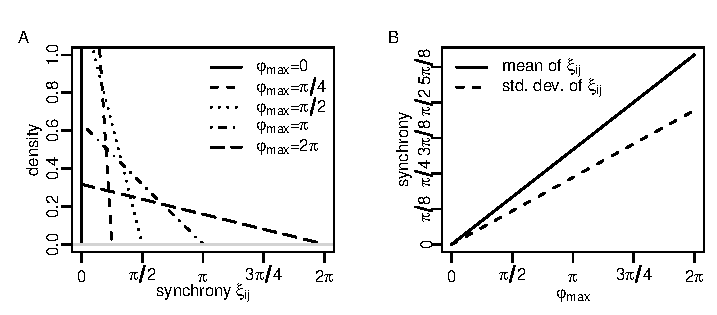
\includegraphics{figure/figure1} \caption{\label{fig:synchrony-1}Synchrony in the case of model 0. (A) distribution
of synchrony $\xi_{ij}$ for various values of $\varphi_{max}$. (B)
mean and standard deviation of the distribution of $\xi_{ij}$ as
functions of $\varphi_{\mbox{\tiny max}}$.}
\end{figure}


Consider that in the metapopulation the phases $\varphi_{i}$ of the
contact rates in the $n$ subpopulations are evenly distributed between
0 and $\varphi_{\mbox{\tiny max}}$ ($0\leqslant\varphi_{\mbox{\tiny max}}\leqslant\pi$).
We can express the mean of the pairwise phase differences $\delta_{ij}=\delta_{ji}$
as 
\begin{equation}
<\!\!\delta_{ij}\!\!>\;=\;<\!\!\delta_{ji}\!\!>\;=2\varphi_{\mbox{\tiny max}}\sum_{k=1}^{n-1}\frac{(n-k)k}{(n-1)n^{2}}=\frac{n+1}{3n}\varphi_{\mbox{\tiny max}}
\end{equation}
 and thus the mean of the synchronies $\xi_{ij}=\xi_{ji}$ as 
\begin{equation}
<\!\!\xi_{ij}\!\!>\;=\;<\!\!\xi_{ji}\!\!>\;=1-\frac{n+1}{3n}\frac{\varphi_{\mbox{\tiny max}}}{\pi}
\end{equation}
 and thus 
\begin{equation}
\lim_{n\to\infty}<\!\!\xi_{ij}\!\!>\;=1-\frac{\varphi_{\mbox{\tiny max}}}{3\pi}
\end{equation}


This last result shows that, for a high enough number $n$ of subpopulations,
the mean value of the $\xi_{ij}$ does not depend on the number of
subpopulation.

The values of $\varphi_{i}$ are chosen so that they are uniformly
distributed between $\varphi_{\mbox{\tiny min}}=0$ and $\varphi_{\mbox{\tiny max}}$.
The distribution of $\xi_{ij}$ doesn't depend on $n$ the number
of subpopulation, but only depends $\varphi_{\mbox{\tiny max}}$ and
may be is characterized by one single parameter (we choose the average
value of all $\xi_{ij}$), view figure \ref{fig:synchrony-1}.

------
\end{document}
